%%%%%%%%%%%%%%%%%%%%%%%%%%%%%%%%%%%%%%%%%%%%%%%%%%%%%%%%%%%%%%%%%%%%%%
% Lớp 10 | Phương pháp tọa độ trong mặt phẳng (𝑂𝑥𝑦) | Đường thẳng trong mặt phẳng tọa độ
% Dạng 0H9?3-7: Bài toán dùng cho tam giác, tứ giác
% Số câu: 11  (sinh tự động bởi tach_cau.py; từ nay thầy sửa trực tiếp file này)
%%%%%%%%%%%%%%%%%%%%%%%%%%%%%%%%%%%%%%%%%%%%%%%%%%%%%%%%%%%%%%%%%%%%%%

%%%%%%%%%%%%%%%% TRẮC NGHIỆM 4 PHƯƠNG ÁN %%%%%%%%%%%%%%%%

% nguồn: MaHoaNH_TracNghiem_Lop10
\begin{ex}%[0H9N3-7]%[ma:5f8e7204]
	Đường thẳng $\Delta\colon 5x+3y=15$ tạo với các trục tọa  độ một tam giác có diện tích bằng bao nhiêu?
	\choice 
		{\True  $7,5$}
		{$5$} 
		 {$15$}
		{$3$} 
	\loigiai{ 
		Ta có $\heva{&\Delta  \cap Ox=A\left(3;0\right)\\&\Delta \cap Oy=B\left(0;5\right)}$.\\
		Vậy $S_{\triangle  OAB}=\dfrac{1}{2} OA\cdot OB=\dfrac{15}{2}=7,5$.
	} 
\end{ex}


%%%%%%%%%%%%%%%% ĐÚNG/SAI %%%%%%%%%%%%%%%%

% nguồn: MaHoaNH_DungSai_Lop10
\begin{ex}%[0H9H3-7]%[0H9H3-4]%[0H9H2-4]%[0H9N1-3]%[ma:a6a4a6db]
	Trong mặt phẳng tọa độ $Oxy$, cho ba điểm $A(1;-1)$, $B(5;-3)$ và $C(2;0)$. Xét tính đúng  sai của mỗi khẳng định dưới đây.
	 \choiceTF
		{\True  Độ dài của đoạn thẳng $AB=\sqrt{20}$}
		{Tọa độ trọng tâm của tam giác $ABC$ là $G\left(\dfrac{8}{3};\dfrac{4}{3}\right)$} 
		 {Tam giác $ABC$ là tam giác vuông tại $A$}
		{\True Diện tích của tam giác $ABC$ là  $3$ (đvdt)}
	\loigiai{ 
		\begin{itemchoice}
			\itemch \textbf{Đúng}. Vì $\overrightarrow{AB}=(4;-2)\Rightarrow AB=\sqrt{4^2+(-2)^2}=\sqrt{20}$. 
			\itemch \textbf{Sai}. Vì tọa độ trọng tâm $G$ của tam  giác $ABC$ là $\heva{&x_{G}=\dfrac{1+5+2}{3}\\&y_{G}=\dfrac{-1+(-3)+0}{3}}
			 \Rightarrow G\left(\dfrac{8}{3};-\dfrac{4}{3}\right)$.
			\itemch \textbf{Sai}. Vì $\heva{&\overrightarrow{AC}=(1;1)\\&\overrightarrow{BC}=(-3;3)} 
			\Rightarrow  \heva{&AC=\sqrt{1^2+1^2}=\sqrt{2}\\&BC=\sqrt{(2-5)^2+(0+3)^2}=\sqrt{18}.}$\\
			Hoặc sử dụng tích vô hướng của 2 vec-tơ $\overrightarrow{AC}\cdot\overrightarrow{BC}=1\cdot (-3)+1\cdot  3=0$.\\
			Suy ra $AC^2+BC^2=AB^2=20$ nên tam giác $ABC$ là tam  giác vuông tại $C$.
			\itemch \textbf{Đúng}. Vì tam giác $ABC$ là tam  giác vuông tại $C$ nên $S_{\triangle ABC}=\dfrac{1}{2}\cdot CA\cdot CB=\dfrac{\sqrt{2}\cdot\sqrt{18}}{2}=3$.
		\end{itemchoice}
	 }
\end{ex}

% nguồn: MaHoaNH_DungSai_Lop10
\begin{ex}%[0H9V3-7]%[ma:3ffaa02b]
	Trong mặt phẳng $Oxy$, cho tam giác $ABC$ có đỉnh $B(-12;1)$ và đường phân giác trong góc $A$ có phương trình $d\colon x+2y-5=0$. Điểm $G\left(\dfrac{1}{3};\dfrac{2}{3}\right)$ là  trọng tâm của $\triangle ABC$.
	 \choiceTF
		{\True Hình chiếu của điểm  $B$ trên đường thẳng $d$ có tọa độ $(-9;7)$}
		{Tung độ điểm $B'$ là điểm đối xứng với $B$ qua đường thẳng $d$ là  một số âm}
		{\True Hai vectơ $\overrightarrow{AB'}$ và $\overrightarrow{B'C}$ cùng  phương với nhau}
		{Có hai điểm $C$ thỏa mãn yêu cầu bài  toán}
	\loigiai{ 
		\begin{itemchoice}
			\itemch Gọi $H(5-2t;t)$, $(t\in \mathbb{R})$ là hình chiếu của điểm  $B$ trên đường thẳng $d$.\\
			Ta có $\overrightarrow{BH}=(17-2t;t-1)$ và $BH\perp d$.\\ 
			Do đó $\overrightarrow{BH}\cdot \overrightarrow{u}_{d}=0\Leftrightarrow(17-2t)\cdot 2-1\cdot(t-1)=0\Leftrightarrow t=7$.\\ 
			Tọa độ điểm $H(-9;7)$. 
			\itemch Gọi $B'$ là điểm đối xứng của $B$ qua  $d$. Khi đó $H$ là trung điểm của $BB'$ nên tọa độ điểm $B'(-6;13)$.
			\itemch Gọi tọa độ điểm $A(5-2a;a)$.\\ 
			Vì $G\left(\dfrac{1}{3};\dfrac{2}{3}\right)$ là  trọng tâm của tam giác $ABC$, suy ra $C(8+2a;1-a)$.\\
			Mặt khác ba điểm  $A$, $B'$, $C$ thẳng hàng nên $\overrightarrow{AB'}$, $\overrightarrow{B'C}$ cùng phương.
			\itemch 
			Ta  có $\overrightarrow{AB'}=(-11+2a;13-a)$, $\overrightarrow{B'C}=(14+2a;-12-a)$.\\
			Suy  ra $\overrightarrow{AB'}$, $\overrightarrow{B'C}$ cùng phương khi và chỉ khi $\dfrac{-11+2a}{14+2a}=\dfrac{13-a}{-12-a}\Rightarrow a=-2$.\\
			Vậy tọa độ điểm  $C(4;3)$.
		\end{itemchoice}
	 }
\end{ex}

% nguồn: MaHoaNH_DungSai_Lop10
\begin{ex}%[0H9V3-7]%[ma:679547e7]
	Trong mặt phẳng $Oxy$, cho tam  giác $ABC$ vuông tại $A(2; 3)$. Đường thẳng qua trung điểm $M$ của $AB$ và vuông góc với $BC$ tại $K(4; 9)$ cắt $AC$ tại $E$ thỏa mãn $KE=2CK$. Biết hoành độ của điểm $M$ lớn hơn $2$.
	 \choiceTF
		{\True Đường  thẳng $BC$ có phương trình là $2x+y-17=0$}
		{Hoành độ của điểm $C$ thỏa mãn yêu cầu  bài toán là một số dương}
		{Có hai điểm $M$ thõa mãn  yêu cầu bài toán}
		{\True  Côsin góc tạo bởi hai vectơ $\overrightarrow{CA}$ và $\overrightarrow{CB}$ bằng $\dfrac{\sqrt{5}}{5}$}
	\loigiai{ 
		\begin{center}
			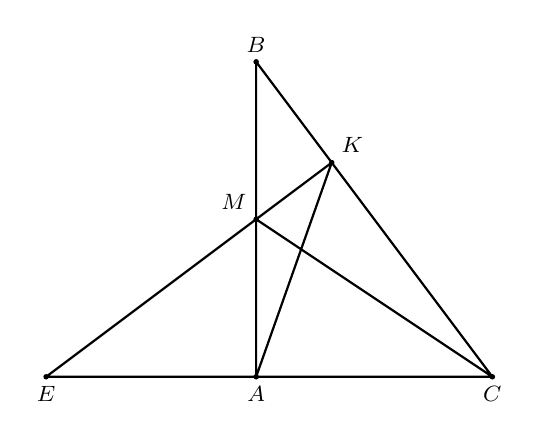
\begin{tikzpicture}[scale=1,font=\footnotesize,line join=round,line cap=round,>=stealth]
					\path (0,0)  coordinate (A) node[below] {$A$}
						(0,4)  coordinate (B) node[above] {$B$}
						(3,0) coordinate (C) node[below] {$C$} 
						(0,2) coordinate (M) node[above left]  {$M$}
						(0.96,2.72) coordinate (K)  node[above right] {$K$}
						(-2.667,0) coordinate (E) node[below]  {$E$};
					\draw[thick] (A)--(B)--(C)--cycle (A)--(K) 
						 (C)--(M)
						 (E)--(K)
						(E)--(A); 
					\foreach \x in {A,B,C,M,K,E} 
					\fill (\x) circle (1pt); 
				\end{tikzpicture}
		\end{center}
	} 
\end{ex}


%%%%%%%%%%%%%%%% TRẢ LỜI NGẮN %%%%%%%%%%%%%%%%

% nguồn: MaHoaNH_TraLoiNgan_Lop10
\begin{bt}%[0H9V3-7]%[ma:01ce2518]
	Trong hệ trục $Oxy$, cho hình thoi $ABCD$. Biết tọa độ điểm $A(3;-1)$, $B(4;2)$ và tâm $I$ của hình thoi  là điểm có hoành độ nguyên, nằm trên đường thẳng $\Delta\colon 2x+y-4=0$. Tính
	 chiều cao từ đỉnh $B$ của tam giác $ABD$? (làm tròn kết quả đến chữ số thập phân thứ hai)
	\shortans{2,53} 
	\loigiai{ 
		\begin{center}
			\begin{tikzpicture}[line join=round,line cap=round,>=stealth,scale=0.75,font=\footnotesize]
					\foreach \x/\y/\n in {0/0/I,4/0/C,-4/0/A,0/-2/B,0/2/D}  \coordinate (\n) at (\x,\y);
					\draw[red] (I)  -- ($(A)!(I)!(B)$) coordinate (H);
					\draw[red] (B)  -- ($(A)!(B)!(D)$) coordinate (K);
					 \draw (A)--(D)--(C)--(B)--(A)
						(B)--(D) 
						(A)--(C); 
					\foreach \t/\g in  {A/180,B/-90,C/0,D/90,H/-100,I/-45}{
						 \fill (\t) circle (1pt) node[shift={(\g:8pt)}]{$ \t $};
					} 
					\draw pic[thin,draw,angle radius=2mm]  {right angle= I--H--A};
					\draw  pic[thin,draw,angle radius=2mm] {right angle= B--K--A};
					\draw pic[thin,draw,angle  radius=2mm] {right angle= B--I--A};
				\end{tikzpicture}
		\end{center}
		Ta có $I$ là tâm của hình thoi  $ABCD$ nên $I$ là trung điểm của $AC$, $BD$ và $AI\perp BI$.\\
		Do $I\in\Delta$ nên  tọa độ $I(a;4-2a)$ và $a\in\mathbb{Z}$.\\
		 Có $\overrightarrow{AI}=(a-3;5-2a)$, $\overrightarrow{BI}=(a-4;2-2a)$.
		\begin{align*}
			AI\perp BI\Rightarrow  \overrightarrow{AI}\cdot\overrightarrow{BI}=0&\Leftrightarrow (a-3)(a-4)+(5-2a)(2-2a)=0\\
			&\Leftrightarrow 5a^2-21a+22=0\Leftrightarrow  \hoac{&a=2\\&a=\dfrac{11}{5}.}
		\end{align*}
		 Với $a=2$ thỏa mãn điều kiện nên $I(2;0)$.\\
		Do $ABCD$ là  hình thoi nên ta có $\mathrm{d}(B,AD)=\mathrm{d}(BC,AD)=\mathrm{d}(CD,AB)=2\mathrm{d}(I,AB)$.
		Phương trình đường thẳng $AB$ có dạng \[\dfrac{x-3}{4-3}=\dfrac{y+1}{2+1}\Leftrightarrow  3(x-3)=y+1\Leftrightarrow 3x-y-10=0.\]
		 Suy ra $\mathrm{d}(B,AD)=2\mathrm{d}(I,AB)=2\cdot\dfrac{|3\cdot2-0-10|}{\sqrt{3^2+1^2}}=\dfrac{8}{\sqrt{10}}=\dfrac{4\sqrt{10}}{10}\approx 2{,}53$.
	} 
\end{bt}

% nguồn: MaHoaNH_TraLoiNgan_Lop10
\begin{bt}%[0H9V3-7]%[ma:248cdd14]
	Trong mặt phẳng với hệ tọa độ $Oxy$, cho tam giác $ABC$. Điểm $M(2;0)$ là trung điểm của $AB$. Đường trung tuyến và đường cao kẻ từ $A$ lần lượt có phương trình $7x-2y-3=0$ và $6x-y-4=0$. Gọi $a$ là hoành độ  và $b$ là tung độ của điểm $C$. Tính giá trị của biểu thức $a+b$.
	 \shortans{-4}
	 \loigiai{
	\immini{Gọi $AH$, $AN$ lần lượt là đường  cao và trung tuyến kẻ từ $A$.\\
		Tọa độ điểm $A$ là nghiệm của hệ phương trình $\heva{&7x-2y-3=0\\&6x-y-4=0}\Leftrightarrow\heva{&x=1\\&y=2}\Rightarrow A(1;2)$.}{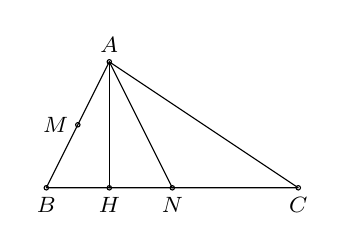
\begin{tikzpicture}[>=stealth,scale=0.8,line join=round,line cap=round,font=\footnotesize]
		 \draw (0,0)--(1,2)--(4,0)--cycle;
		 \draw (1,2)--(1,0);
		\draw  (1,2)--(2,0);
		\draw (1,2)  node[above]{$A$};
		 \foreach \x in {(1,2),(0,0),(1,0),(2,0),(4,0)}{\draw \x circle (1pt);}
		\draw (0,0) node[below]{$B$}; 
		\draw  (1,0) node[below]{$H$};
		\draw  (2,0) node[below]{$N$};
		\draw (4,0)  node[below]{$C$};
		\draw (0.5,1) circle (1pt)  node[left]{$M$};
	\end{tikzpicture}
		 }
		\noindent $M$ là trung điểm của $AB$  nên ta có
		 \[
		\heva{&x_M=\dfrac{x_A+x_B}{2}\\&y_M=\dfrac{y_A+y_B}{2}}\Rightarrow\heva{&x_B=2x_M-x_A=2\cdot 2-1=3\\&y_B=2y_M-y_A=2\cdot  0-2=-2}\Rightarrow B(3;-2).
		 \]
		$BC$ vuông góc với  $AH$ nên có phương trình $x+6y+c=0$.\\
		Đường thẳng $BC$ đi  qua $B$ nên
		\[ 
		3+6\cdot(-2)+c=0\Leftrightarrow c=9. 
		 \]
		 Suy ra phương trình $BC$ là $x+6y+9=0$.\\
		Tọa độ điểm $N$ là nghiệm của  hệ phương trình
		 \[
		\heva{&7x-2y-3=0\\&x+6y+9=0}\Leftrightarrow \heva{&x=0\\&y=-\dfrac{3}{2}}\Rightarrow N\left(0;-\dfrac{3}{2}\right). 
		\] 
		Từ $N$ là trung điểm của $BC$ suy ra tọa độ điểm $C(-3;-1)$.\\ 
		 Do đó $\heva{&a=-3 \\&b=-1 }\Rightarrow a+b=-4$.
	 }
\end{bt}

% nguồn: MaHoaNH_TraLoiNgan_Lop10
\begin{bt}%[0H9C3-7]%[ma:36724f39]
	Trong mặt phẳng $Oxy$, cho điểm $M(1; 2)$ và đường thẳng $\Delta\colon 2 x-y-5=0$, $A$ là điểm thuộc  đường thẳng $\Delta$ sao cho độ dài $MA$ ngắn nhất. Diện tích tam giác $MAO$ bằng bao nhiêu (kết quả được viết dưới dạng thập phân).
	 \shortans{2,5}
	 \loigiai{
		\begin{center}
			\begin{tikzpicture}[line cap=round,line join=round,font=\footnotesize,>=stealth,scale=1.4]
					\path 
						(0,0)  coordinate (O)
						 (1,0) coordinate (A)
						(6,0) coordinate  (B)
						(3,1) coordinate (M) 
						 ($(A)!(M)!(B)$) coordinate (H);
					 \draw (O)--(B)
						(A)--(M)--(H); 
					 \foreach \x/\g in {A/-90,M/90,H/-90}{
						\fill  (\x) circle (0.8pt) node[shift=(\g:4mm)] {$\x$};}
					\draw pic  [draw,angle radius=3mm] {right angle = B--H--M};
				\end{tikzpicture}
		\end{center}
		 Gọi $H$ là hình chiếu vuông góc của điểm $M$ lên đường thẳng $\Delta$.\\
		Đường thẳng đi qua điểm $M(1; 2)$ và vuông góc với đường thẳng $\Delta$ có phương trình  là $x+2 y-5=0$.\\
		Tọa độ điểm $H$ là nghiệm của hệ phương trình $\heva{&2 x-y-5=0 \\ &x+2 y-5=0 }  \Rightarrow H(3; 1)$.\\
		Xét tam giác $AMH$ vuông tại $H$, ta có  $MA \geq MH$ suy ra độ dài $M A$ ngắn nhất khi $A \equiv H$ suy ra $A(3; 1)$.\\
		Khi đó  ta có $\overrightarrow{O A}=(3; 1) \Rightarrow \left|\overrightarrow{O A}\right|=\sqrt{10}$.\\
		 Đường thẳng $O A$ có phương trình là $x-3 y=0$.\\
		Ta có khoảng cách từ điểm $M$ đến đường thẳng $OA$  là $\mathrm{d}(M; O A)=\dfrac{\left|1-3\cdot 2\right|}{\sqrt{10}}=\dfrac{5}{\sqrt{10}}$.\\
	 Vậy diện tích tam giác $MAO$ là $S=\dfrac{1}{2} \cdot \mathrm{d}(M; O A) \cdot O A=\dfrac{1}{2} \cdot \dfrac{5}{\sqrt{10}} \cdot \sqrt{10}=\dfrac{5}{2}$.}
\end{bt}


%%%%%%%%%%%%%%%% TỰ LUẬN %%%%%%%%%%%%%%%%

% nguồn: MaHoaNH_TuLuan_Lop10
\begin{bt}%[0H9V3-7]%[ma:6f588310]
	Trong mặt phẳng $Oxy$, cho đường thẳng $d\colon y=ax+b$ đi qua điểm $K(1;3)$ và $d$ tạo với hai tia $Ox$, $Oy$ một tam giác có diện tích bằng $6$. Tính giá trị của biều  thức $b-a$.
	 \loigiai{
		Gọi  phương trình đường thẳng $d\colon y=ax+b$.\\
		Vì đường thẳng $d$ đi qua điểm $K(1;3)$ nên $a+b=3$.\\ 
		Đường  thẳng $d\colon y=ax+b$ cắt hai tia $Ox$, $Oy$ lần lượt là $A\left(-\dfrac{b}{a};0\right)$, $B(0;b)$, $(a<0,b>0)$.\\
		Theo  giả thiết $S_{\triangle OAB}=\dfrac{1}{2}OA\cdot OB=\dfrac{1}{2}\cdot\left|\dfrac{b}{a}\right|\cdot|b|=-\dfrac{b^2}{2a}=-\dfrac{b^2}{2(3-b)}$.\\
		Do $S_{\triangle OAB}=6$ nên  $-\dfrac{b^2}{2(3-b)}=6\Leftrightarrow b^2-12b+36=0\Leftrightarrow b=6$.\\
		Suy ra  $a=-3$ nên $b-a=9$.
	 }
\end{bt}

% nguồn: MaHoaNH_TuLuan_Lop10
\begin{bt}%[0H9V3-7]%[ma:7ca2b89b]
	 Trong mặt phẳng $Oxy$ cho tam giác $ABC$ có tọa độ các đỉnh $A(1;1)$, $B(-2;5)$. Đỉnh $C$ thuộc đường thẳng $d\colon x-4=0$, trọng tâm $G$ của tam giác $ABC$ thuộc đường thẳng $d'\colon 2x-3y+6=0$. Tính diện tích tam giác $ABC$.
	\loigiai{ 
		Đỉnh $C$ thuộc đường thẳng $d\colon x-4=0\Rightarrow C(4;b)$.\\ 
		$G \in d'\colon 2x-3y+6=0\Rightarrow  G\ \left(a;\dfrac{2a+6}{3}\right)$.\\
		Vì  $G$ là trọng tâm của tam giác $ABC$ nên
		$\heva {&1-2+4=3a\\&1+5+b=2a+6}\Rightarrow \heva {&a=1\\&b=2}\Rightarrow C(4;2)$,  $G(1;\dfrac{8}{3})$.\\
		Ta có phương trình  đường thẳng $(AB) \colon 4x+3y-7=0$ và $AB=5$; $\mathrm{d}(C, (AB))=3$.\\
		Vậy  diện tích tam giác $ABC$ là $S_{ABC}=\dfrac{1}{2}AB\cdot \mathrm{d}(C, (AB))=\dfrac{15}{2}=7{,}5$.
	} 
\end{bt}

% nguồn: MaHoaNH_TuLuan_Lop10
\begin{bt}%[0H9V3-7]%[ma:a87820ca]
	Cho tam giác $ABC$ biết $A(1; 4)$, $B(3;-1)$, $C(6;-2)$. Phương trình đường thẳng $d$ qua $C$  và chia tam giác thành hai phần, sao cho phần chứa điểm $A$ có diện tích gấp đôi phần chứa điểm $B$ có dạng $ax+bx+c=0$. Tính $a+b+c$ ?
	\loigiai{ 
	\immini{Gọi $D$ là giao điểm của đường thẳng  $d$ và đoạn thẳng $AB$.\\
		Gọi $H$ là hình chiếu vuông  góc của $C$ trên $AB$.\\
		Ta có $S_{\triangle ACD}=\dfrac{1}{2} CH \cdot A D$ và $S_{\triangle BCD}=\dfrac{1}{2}  CH \cdot BD$.\\
		Vì $S_{\triangle ACD}=2  S_{\triangle BCD} \Rightarrow AD=2 BD$.\\
		Mà $D\in AB$ nên $\overrightarrow{AD}=2 \overrightarrow{BD}$.}{\begin{tikzpicture}[>=stealth,line join=round,line cap=round,font=\footnotesize,scale=1]
		 \path (0,0) coordinate (A)
			(4,0) coordinate  (B)
			(50:3) coordinate (C) 
			($(A)!2/3!(B)$) coordinate  (D)
			($(A)!(C)!(B)$) coordinate  (H);
		 \draw (A)--(B)--(C)--cycle
			 (H)--(C)--(D);
		\foreach  \x/\g in {A/-90,B/-90,C/90,D/-90,H/-90}\fill[black](\x) circle (1pt)+(\g:.3) node{$\x$};
	\end{tikzpicture}
		 }
		 \noindent
		 Suy ra $\heva{&x_D-1=2(x_D-3)\\&y_D-4=2(y_D+1)}\Leftrightarrow\heva{&x=\dfrac73\\&y=\dfrac23}\Rightarrow D\left(\dfrac73;\dfrac23\right)$.\\
		Ta có đường thẳng $d$ đi qua $C(6;-2)$ và nhận $\overrightarrow{CD}=(-11;8)$ làm vectơ chỉ phương nên đường thẳng $d$ có vectơ pháp tuyến  là $\overrightarrow{n}=(8;11)$.\\
		 Suy ra phương trình đường thẳng $d$ có dạng $8x+11y-26=0$ nên $\heva{&a=8\\&b=11\\&c=-26.}$\\
		Vậy $a+b+c=8+11-26=-7$. 
	} 
\end{bt}

% nguồn: MaHoaNH_TuLuan_Lop10
\begin{bt}%[0H9C3-7]%[ma:8c3d151d]
	\immini[thm]{Một ao cá có dạng hình chữ nhật $ABCD$ với chiều dài $AD=17$\,m, chiều rộng $AB=13$\,m. Phần tam giác $DEF$ người ta để  nuôi vịt, biết $AE=6$\,m, $CF=6{,}5$\,m (minh họa như hình vẽ). Tính khoảng cách từ vị trí người đứng ở vị trí $B$ câu cá đến vách ngăn nuôi vịt là đường thẳng $EF$ (kết quả làm tròn đến hàng phần chục).}
	{\begin{tikzpicture}[scale=0.5,font=\footnotesize,line join = round,line cap = round,>=stealth]
		\path 
			 (-4,0) coordinate (B)
			(-4,7)  coordinate (A)
			(3,0) coordinate (C) 
			 (3,7) coordinate (D)
			 (-5/3,7) coordinate (E)
			 (3,3.5) coordinate (F);
		 \draw[fill=black!30!green,opacity=0.6]
			 (-5,-1.5)
			.. controls ++(90:0.1)  and ++(180: 1).. (-5,8)
			 .. controls ++(180:0.1) and ++(90: 1).. (5.5,8)
			.. controls ++(90:0.1)  and ++(100: 1).. (5.5,-1.5)
			 .. controls ++(180:0.1) and ++(30: 1).. (-5,-1.5);
		 \draw[fill=green!50] plot[smooth cycle] coordinates{(5.11,1.14)
			 (5.87,1.01)
			 (6.09,1.88)
			 (5.93,2.62)
			(6.03,3.31) 
			 (5.5,3.65)
			 (5.37,4.45)
			 (5,5)
			 (4.66,4.29)
			 (4.29,3.55)
			(4.5,2.88) 
			(3.94,2.62) 
			(3.81,1.8) 
			(4.23,1.24) 
			(4.82,1.19)}; 
		\draw[fill=black!70] plot[smooth]  coordinates{(5.3,0)
			 (5.25,1.14)
			 (5.25,1.8)
			 (5.7,2.9)
			(5.18,2.05) 
			 (5.09,4.2)
			(5.06,2.3) 
			(5.0,1.65) 
			 (4.2,2.4)
			(5.01,1.29) 
			(5,0)}; 
		 \fill[cyan!30] (-4,0) rectangle (3,7);
		 \draw (A)--(B)--(C)--(D)--cycle;
		 \draw[red] (E)--(F);
		\node[scale=2.3,yscale=2] at  (-4.2,1){\faBlind};
		 \draw (-3.5,-0.4)
			..  controls ++(30:0.1) and ++(70: 1).. (-2,1);
		\foreach \y in  {0,60,...,720}{
			 \draw[color=white] (0.5,6.5)--++(\y:.1)
			 (1.5,6.5)--++(\y:.1)
			(2.5,6.5)--++(\y:.1) 
			(1,5.7)--++(\y:.1) 
			(2,5.7)--++(\y:.1) 
			 (2.7,5.7)--++(\y:.1)
			 (1.8,4.7)--++(\y:.1)
			 (2.6,4.7)--++(\y:.1);}
		\foreach \p/\r in {B/-90,C/-90,F/0,D/60,E/90,A/110} 
		\fill[color=white] (\p) circle (1.5pt) node[shift={(\r:3mm)}]{$\p$}; 
	\end{tikzpicture}
	} 
	\loigiai{ 
		Chọn hệ trục tọa độ $Oxy$, có điểm $O$ trùng với điểm $B$, các tia $Ox$,  $Oy$ tương ứng trùng với các tia $BC$, $BA$. Chọn $1$ đơn vị độ dài trên mặt phẳng tọa độ tương ứng với $1$\,m trong thực tế.
		\begin{center}
			\begin{tikzpicture}[scale=0.5,font=\footnotesize,line join = round,line cap = round,>=stealth]
					\path 
						 (-4,0) coordinate (B)
						 (-4,7) coordinate (A)
						(3,0) coordinate (C) 
						(3,7) coordinate (D) 
						 (-5/3,7) coordinate (E)
						(3,3.5)  coordinate (F);
					\draw[fill=black!30!green,opacity=0.6] 
						(-5,-1.5) 
						.. controls ++(90:0.1)  and ++(180: 1).. (-5,8)
						.. controls ++(180:0.1) and ++(90: 1).. (5.5,8) 
						.. controls  ++(90:0.1) and ++(100: 1).. (5.5,-1.5)
						 .. controls ++(180:0.1) and ++(30: 1).. (-5,-1.5);
					\draw[fill=green!50]  plot[smooth cycle] coordinates{(5.11,1.14)
						 (5.87,1.01)
						(6.09,1.88) 
						(5.93,2.62) 
						(6.03,3.31) 
						 (5.5,3.65)
						(5.37,4.45) 
						(5,5) 
						 (4.66,4.29)
						(4.29,3.55) 
						(4.5,2.88) 
						(3.94,2.62) 
						 (3.81,1.8)
						 (4.23,1.24)
						 (4.82,1.19)};
					 \draw[fill=black!70] plot[smooth] coordinates{(5.3,0)
						 (5.25,1.14)
						 (5.25,1.8)
						(5.7,2.9) 
						 (5.18,2.05)
						 (5.09,4.2)
						(5.06,2.3) 
						 (5.0,1.65)
						 (4.2,2.4)
						 (5.01,1.29)
						(5,0)}; 
					\fill[cyan!30]  (-4,0) rectangle (3,7);
					 \draw (A)--(B)--(C)--(D)--cycle;
					\draw[red] (E)--(F); 
					\node[scale=2.3,yscale=2] at (-4.2,1){\faBlind}; 
					 \draw (-3.5,-0.4)
						.. controls ++(30:0.1) and ++(70:  1).. (-2,1);
					\foreach \y in {0,60,...,720}{ 
						\draw[color=white]  (0.5,6.5)--++(\y:.1)
						 (1.5,6.5)--++(\y:.1)
						(2.5,6.5)--++(\y:.1) 
						 (1,5.7)--++(\y:.1)
						(2,5.7)--++(\y:.1) 
						(2.7,5.7)--++(\y:.1) 
						 (1.8,4.7)--++(\y:.1)
						(2.6,4.7)--++(\y:.1);} 
					\foreach \p/\r  in {B/-90,C/-90,F/0,D/60,E/90,A/110}
					\fill[color=white] (\p) circle  (1.5pt) node[shift={(\r:3mm)}]{$\p$};
					\draw[->]  (-6,0)--(7,0) node[above]{$x$};
					\draw[->] (-4,-2)--(-4,10)  node[left]{$y$};
				\end{tikzpicture}
		\end{center}
		Khi đó $A(0;13)$,  $B(0;0)$, $C(17;0)$, $D(17;13)$, $E(6;13)$, $F(17;6{,}5)$,
		 $\overrightarrow{EF}=(11;-6{,}5)$.\\
		Đường thẳng $EF$  có vectơ chỉ phương là $\overrightarrow{EF}=(11;-6{,}5)$ nên có vectơ pháp tuyến $\overrightarrow{n}=(6{,}5;11)$ và đi qua điểm $E(6;13)$.\\
		Suy ra phương trình tổng quát  của đường thẳng $EF$ là
		\[6{,}5(x-6)+11(y-13)= 0\Leftrightarrow 6{,}5x+11y-182=0.\] 
		Khoảng cách từ $B$ đến  đường thẳng $EF$ là $\mathrm{d}(B,EF)=\dfrac{|-182|}{\sqrt{6{,}5^2+11^2}} \approx 14{,}24$.\\
		Vậy khoảng cách từ vị trí người đứng ở vị trí $B$  câu cá đến vách ngăn nuôi vịt là đường thẳng $EF$ bằng $14{,}24$ mét.
	} 
\end{bt}
